\chapter{APK súbory}
\label{APKsubory}
APK súbory sú balíčky používané operačným systémom Android. Celý názov ukrytý za skratkou APK je Android application package file. Tieto súbory slúžia na distribúciu aplikácií v operačnom systéme Android. Ich použitie a význam je analogický ako pri MSI\footnote{\url{Windows Installer Package https://technet.microsoft.com/en-us/library/cc978328.aspx}} balíčkoch používaných v systéme Microsoft Windows, alebo DEB\footnote{\url{https://www.debian.org/doc/manuals/debian-faq/ch-pkg\_basics.en.html}} balíčkoch používaných v niektorých linuxových distribúciách. APK súbory sú asociované s príponou .apk a príslušný MIME typom \zv{application/vnd.android.package-archive}.

Štruktúra APK balíčkov vychádza z JAR\footnote{Java archive} balíčkov -- súborov používaných na distribúciu aplikácií alebo knižníc na platforme Java. Formát APK rozširuje všeobecnejší JAR formát o súbory, ktoré sú špecifické pre cieľovú platformu, ktorou je operačný systém Android. Zároveň si však ponecháva vlastnosti JAR súborov. APK balíčky sú archívne súbory v ZIP\footnote{\url{https://en.wikipedia.org/wiki/Zip\_(file_format)}} formáte.  Keďže APK používajú ZIP formát, k ich obsahu môžeme jednoducho pristúpiť rozbalením archívu štandardným spôsobom.  APK súbory vznikajú ako výstup kompletnej kompilácie a zabalenia aplikácií pre Android. APK súbor každej aplikácie obsahuje všetky potrebné súbory na jej inštaláciu a spustenie. Medzi týmito súbormi sa typicky nachádza \zv{classes.dex} súbor obsahujúci skompilovaný zdrojový kód, \zv{resources.arsc} súbor ktorý obsahuje skompilované zdroje aplikácie, súbor \zv{AndroidManifest.xml} a neskompilované súbory ako sú napríklad obrázky.\\\\
\begin{figure}[htb]
  \begin{center}
    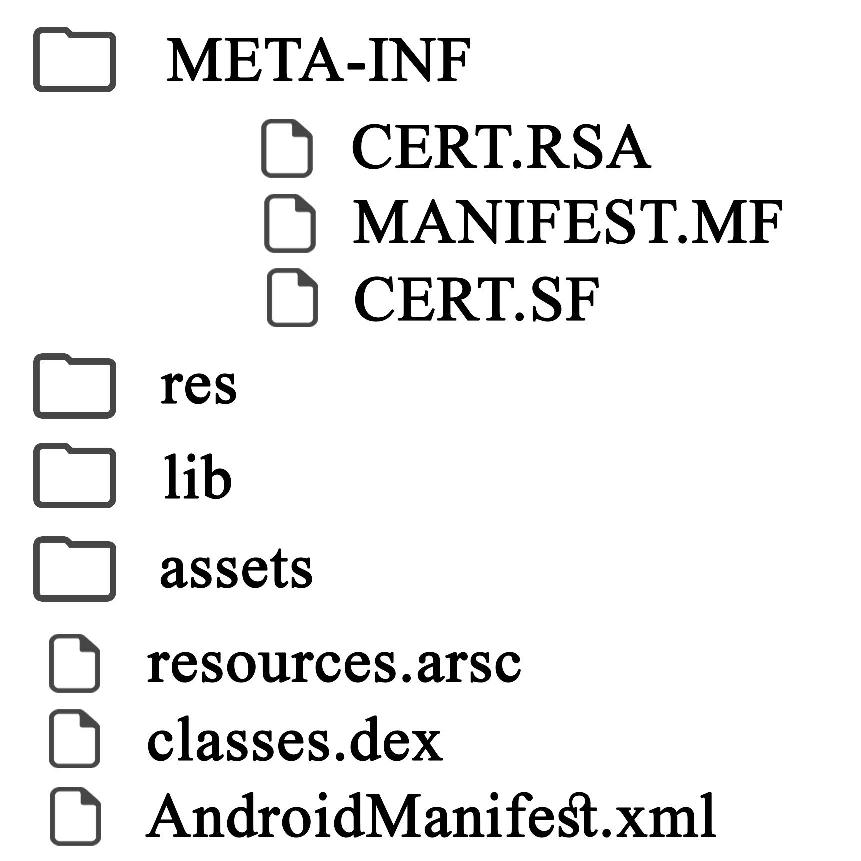
\includegraphics[width=60mm]{images/apkStructure.pdf}
  \end{center}
  \caption{Typická štruktúra APK súboru}
\end{figure}

\section{Priečinok META-INF}
\label{META-INF}
Priečinok obsahujúci súbory, ktorých úlohou je zaručiť integritu ostatných súborov v APK balíčku a s ňou spojenú bezpečnosť celého systému. V prípade detekcie pozmenených súborov a narušenia integrity operačný systém Android nedovolí inštaláciu APK balíčku. Po každej zmene je nutné balíček digitálne podpísať.


\subsection*{CERT.RSA}
\label{CERT.RSA} 
Súbor obsahujúci verejný kľúč ktorý slúži na overenie digitálneho podpisu balíčka.
\subsection*{MANIFEST.MF}
\label{MANIFEST.MF}
Súbor obsahujúci relatívne cesty a SHA-1 hashe \footnote{reťazce v Base64 kódovaní} všetkých súborov v APK balíčku. Tento súbor neobsahujú len APK súbory, je typický pre každý JAR archív.\\\\
Typický začiatok súboru \zv{MANIFEST.MF} vyzerá nasledovne: \\

\begin{verbatim}
Manifest-Version: 1.0
Built-By: 0.12.2
Created-By: Android Gradle 0.12.2

Name: res/drawable-xhdpi-v4/libraries.png
SHA1-Digest: VvgaO1jpW3iS1nBBikD/urdbN58=

Name: res/layout/activity_settings.xml
SHA1-Digest: 1coP1lt9Lmccc7SMZGHxNv4bbKs=
\end{verbatim}

\subsection*{CERT.SF}
\label{CERT.SF}
Súbor podobný ako \zv{MANIFEST.MF}, avšak namiesto SHA-1 hashov samotných súborov obsahuje SHA-1 hashe záznamov o týchto súboroch z \zv{MANIFEST.MF}. Okrem toho obsahuje aj hash celého súboru \zv{MANIFEST.MF}. \newline Záznam o jednom súbore v APK balíčku v súbore \zv{CERT.SF} vyzerá nasledovne: \newline
\begin{verbatim}
Name: res/drawable-xhdpi-v4/libraries.png
SHA1-Digest: Slg56lqothjvmaBikD/urdb7q6=
\end{verbatim}\mbox{}\\
Reťazec \zv{Slg56lqothjvmaBikD/urdb7q6=} reprezentuje SHA-1 hash nasledujúceho záznamu zo súboru \zv{MANIFEST.MF}:\mbox{}\\
\begin{verbatim}
“Name: res/drawable-xhdpi-v4/libraries.png
SHA1-Digest: VvgaO1jpW3iS1nBBikD/urdbN58=
”\end{verbatim}

\section{Priečinok res}
\label{res}
Priečinok obsahujúci zdrojové súbory ako napríklad obrázky, zvuky alebo ikony. Okrem multimediálnych súborov obsahuje taktiež zdrojové XML súbory určujúce vzhľad obrazoviek, použité grafické štýly, alebo texty použité v aplikácii. Niektoré z týchto XML súborov môžu byť skompilované do binárneho formátu. V zdrojovom kóde sú tieto zdroje odkazované pomocou unikátnych identifikátorov. Identifikátory sú generované počas kompilácie nástrojom aapt a nachádzajú sa v projektovej triede \zv{R}. Pre každý typ zdrojového súboru je generovaná podtrieda triedy \zv{R}. Všetky zdroje aplikácie by mali byť externalizované a uložené v špecifickom podpriečinku v tomto adresári. \\\\
\textbf{Podporované podpriečinky}
\begin{itemize}
\item animator - obsahuje XML súbory definujúce property animácie\cite{article-full}
\item anim - obsahuje XML súbory definujúce tween animácie, môže obsahovať aj property animácie
\item color - obsahuje XML súbory definujúce farby a ich zmeny na základe stavu objektov na ktoré sú aplikované
\item drawable - obsahuje obrázky vo formáte PNG, 9.PNG, JPG, GIF alebo XML súbory skompilované do formy vykresliteľných obrázkov
\item mipmap - ikony aplikácie s rôznou hustotou pixelov
\item layout - obsahuje súbory vo formáte XML definujúce vzhľad rozmiestnenie prvkov na obrazovke
\item menu - obsahuje súbory XML definujúce menu aplikácie
\item raw - obsahuje súbory ktoré musia byť uložené a použité v neskomprimovanej forme a kvalite
\item values - obsahuje súbory vo formáte XML definujúce hodnoty textových reťazcov, farieb, štýlov, základných rozmerov
\item xml - obsahuje XML súbory, ktoré môžu byť načítané počas behu aplikácie
\end{itemize}

\noindent V spomenutých priečinkoch sú uložené základné zdroje aplikácie. Tieto zdrojové súbory určujú základný dizajn a obsah aplikácie. Avšak rôzne typy Android zariadení môžu využívať rôzne zdrojové súbory. Alternatívne zdroje sa využívajú na prispôsobenie dizajnu a obsahu veľkosti a aktuálnej konfigurácií zariadenia. Sú umiestnené v priečinku, ktorého názov pozostáva z typu zdrojového súboru, ktorý korešponduje so základným názvom priečinku a názvu hodnoty konfiguračného atribútu pre ktorý je tento priečinok určený. Je možné kombinovať viacero konfiguračných atribútov.\\\\
\textbf{Najpoužívanejšie atribúty}
\begin{itemize}
\item Jazyk a región – jazyk je definovaný podľa ISO 639-1\footnote{http://www.iso.org/iso/home/standards/language\_codes.htm} kódovania s možnosťou rozšírenia pomocou ISO 3166-1-alpha-2 regionálneho kódu. Napríklad obrázky špecifické pre zariadenia s francúzskym jazykom sa nachádzajú v priečinku \cesta{res/drawable-fr}
\item Veľkosť obrazovky –  v závislosti na veľkosti a rozlíšení obrazovky rozlišuje štyri možné hodnoty -- small, normal, large, xlarge
\item Orientácia obrazovky – v závislosti na orientácii zariadenia hodnota port pre zariadenie vo vertikálnej polohe, hodnota land pre polohu horizontálnu
\item Hustota obrázkových bodov obrazovky -  hodnoty určujúce vhodnosť zdrojových súborov vzhľadom na hustotu obrázkových bodov obrazovky daného zariadenia
\end{itemize}


\section{Priečinok lib}
\label{lib}
Priečinok obsahujúci skompilovaný zdrojový kód natívnych knižníc. Tieto knižnice sú špecifické pre typ procesora. V závislosti na architektúre procesora obsahuje podpriečinky : \zv{armeabi, armeabi-v7a, arm64-v8a, x86, x86\_64, mips}.

\section{Priečinok assets}
\label{assets}
Priečinok obsahujúci súbory uložené a používané v originálnej neskomprimovanej forme. V tomto priečinku sa často nachádzajú textové súbory, html súbory, licenčné informácie, obrázky alebo textúry. Na rozdiel od priečinku \cesta{res/raw/}, zdrojovým súborom v umiestneným v priečinku assets nie sú pridelené unikátne identifikátory uložené v triede \zv{R.java}. K súborom sa pristupuje ako k dátam uloženým v bežnom súborovom systéme. Trieda \zv{AssetManager} poskytuje funkcionalitu na čítanie súborov ako prúdu bytov a  navigovanie v tomto priečinku.

\section{resources.arsc}
\label{resources.arsc}
Súbor obsahujúci mapovanie medzi zdrojovými súbormi  z priečinku \zv{res} a ich identifikátormi.  Vytvára sa počas kompilácie. Obsahuje XML súbory v binárnom formáte.

\section{classes.dex}
\label{classes.dex}
\zv{Classes.dex} je súbor obsahujúci skompilovaný zdrojový kód aplikácie.  Zdrojové súbory Android aplikácií sú napísané v jazyku Java. Java súbory sú skompilované do Java bytekódu pomocou bežného kompilátoru pre platformu Java. Výsledkom tejto kompilácie sú súbory s príponou \zv{class}, ktoré sú následne preložené do Dalvik bytekódu pomocou nástroja \zv{dx} ktorý je súčasťou Android Software Developement Kit. Výstupom nástroju \zv{dx} je jediný súbor obsahujúci skompilovaný celý výkonný zdrojový kód aplikácie -- \zv{classes.dex}. Tento súbor je skomprimovanou a optimalizovanou verziou všetkých \zv{class} súborov. Takto skompilovaný program môže byť vykonaný len vo virtuálnom stroji Dalvik, alebo v novšom prostredí ART (Android Runtime) používanom primárne od verzie Android 5.0 „Lollipop“.

\section{AndroidManifest.xml} 
\label{AndroidManifest.xml}
http://developer.android.com/guide/topics/manifest/manifest-intro.html
Súbor ktorý musí obsahovať každá Android aplikácia. Tento súbor poskytuje informácie o aplikácii operačnému systému Android. Neobsahuje žiadny výkonný kód. Definuje meno a verziu, ktoré slúžia ako unikátny identifikátor danej aplikácie. Popisuje všetky komponenty z ktorých sa aplikácia skladá, cesty k použitým knižniciam, minimálny vyžadovaný level Android API, oprávnenie vyžadované aplikáciu na prístup k chráneným častiam Android API a taktiež oprávnenia, ktoré sú vyžadované od iných komponent pri pokuse komunikovať s danou aplikáciou. Súbor \zv{AndroidManifest.xml}, ktorý nájdeme v APK balíčku je vo formáte binárneho XML súboru. Je ho však možné previesť do klasického čitateľného XML formátu.

Keďže \zv{AndroidManifest.xml} je základným súborom poskytujúcim metadáta o Android aplikácii a APK súbore, informácie získané z tohto súboru tvoria veľkú časť štatistických dát zbieraných a vyhodnocovaných v tejto práci. Preto sa detailnejšie pozrieme na jeho štruktúru a niektoré dôležité elementy, ktoré obsahuje.\\ Nasledujúci diagram ukazuje základnú štruktúru tohto XML súboru.
\begin{lstlisting} [language=XML, caption= {Základná štruktúra súboru AndroidManifest.xml}]
<?xml version="1.0" encoding="utf-8"?>
<manifest>
    <uses-permission />
    <permission />
    <uses-sdk />
    <uses-configuration />  
    <uses-feature />  
    <supports-screens />  
    <compatible-screens />  
    <application>
        <activity />
        <service/>
        <receiver/>
        <provider/>
        <uses-library />
    </application>
</manifest>
\end{lstlisting}

\subsection{Element manifest}
\label{el_manifest}
\lstset{language=XML}
\begin{lstlisting}
<manifest xmlns:android="URL"
          package="string"
          android:sharedUserId="string"
          android:sharedUserLabel="string resource"
          android:versionCode="integer"
          android:versionName="string"
          android:installLocation=["auto" | "internalOnly" |
                                        "preferExternal"] >
</manifest>
\end{lstlisting}
\zv{AndroidManifest.xml} obsahuje element manifest ako koreňový prvok. Tento element je povinný a každý manifest ho obsahuje práve jeden. \newline\newline
\noindent Element manifest definuje atribúty:\\
\begin{itemize}
\item xmlns:android – povinný atribút definujúci menný priestor
\item package – meno balíku aplikácie, povinný atribút definujúci identitu aplikácie. Meno balúku nemôže byť zmenené
\item android:sharedUserId – identifikátor aplikácie zdieľaný s ostatnými aplikáciami za účelom vzájomnej komunikácie
\item android:sharedUserLabel – čitateľná podoba android:sharedUserId identifikátoru
\item android:versionCode – interná informácia o verzii aplikácie. Tento atribút je využívaný len na rozoznanie novších verzíí od starších. Novšie aplikácie obsahujú vyššiu hodnotu
\item android:versionName – informácia o verzií aplikácie prezentovaná užívateľom. Pre systém Android neposkytuje informáciu o verzií aplikácie, tú obsahuje atribút android:versionCode.
\item android:installLocation – určuje miesto základné miesto inštalácie aplikácie. Pokiaľ je aplikáciu možné nainštalovať len do vnútornej pamäti zariadenia, obsahuje hodnotu internalOnly. Takáto aplikácia nemôže byť presunutá na externé pamäťové médium (typicky SD karta). Táto hodnota je základnou použitou možnosťou, ak tento atribút nie je definovaný. V prípade hodnoty auto sú aplikácie inštalované vo vnútornej pamäti, ale môžu byť presunuté do pamäti externej. Hodnota preferExternal zabezpečí, že systém sa pokúsi o inštaláciu na externé pamäťové médium. V prípade neúspechu sa použije interná pamäť
\end{itemize}

\subsection{Element uses-permission}
\label{el_uses-permission}
\lstset{language=XML}
\begin{lstlisting}
<uses-permission android:name="string"
        android:maxSdkVersion="integer" />
\end{lstlisting}
Prístup k niektorým dátam alebo častiam kódu je z dôvodu ochrany limitovaný. Android využíva princíp povolení\footnote{angl. permissions}. Povolenia môžu byť definované samotnou aplikáciou, inou aplikáciou alebo systémom Android. Aplikácia, ktorá chce pristupovať k chráneným dátam alebo používať chránené časti kódu, musí pomocou tagu uses-permissions deklarovať vyžadované povolenia. Prístupové povolenia sú aplikácii schválené užívateľom. Vo verzii Android 5.1 a starších, systém počas inštalácie oboznámi užívateľa so všetkými povoleniami, ktoré aplikácia vyžaduje. V prípade, že ich používateľ neschváli, aplikácia nebude nainštalovaná. Od verzie Android 6.0 užívateľ schvaľuje povolenia počas behu aplikácie.\\\\ 
Element uses-permission definuje atribúty:\\
\begin{itemize}
\item android:name – definuje názov povolenia
\item android:maxSdkVersion – najvyšší level Android API, pre ktorý je dané povolenie potrebné
\end{itemize}

\subsection{Element permission}
\lstset{language=XML}
\begin{lstlisting}
<permission android:description="string resource"
            android:icon="drawable resource"
            android:label="string resource"
            android:name="string"
            android:permissionGroup="string"
            android:protectionLevel=["normal"|"dangerous"| 
                                     "signature"|
                                     "signatureOrSystem"] />
\end{lstlisting}
Definuje bezpečnostné povolenie, ktoré môže byť použité na obmedzenie prístupu ku komponente aplikácie. Toto povolenie je následne používané aplikáciami, ktoré vyžadujú prístup k chránenej časti danej aplikácie.\\\\ Najdôležitejšie atribúty definované v rámci elementu permission:\\
\begin{itemize}
\item android:name – názov povolenia, aplikácie vyžadujúce dané povolenie uvádzajú túto hodnotu v atribúte android:name v tagu uses-permission. Názov musí byť unikátny a mal by dodržiavať konvencie pomenovávania jazyka Java.
\item android:permissionGroup – priradí toto povolenie do skupiny povolení (angl. Permission group). Táto skupina povolení musí byť deklarovaná v rámci elementu permission-group v niektorej z nainštalovaných aplikácií. Slúži na logické zoskupenie významovo podobných oprávnení.
\item android:protectionLevel – charakterizuje potenciálne riziko spojené s použitím daného povolenia. Táto hodnota určuje postup operačného systému pri rozhodovaní o udelení povolenia. 
Základnou hodnotou je „normal“, ktorá reprezentuje povolenia s nízkou mierou rizika. Tieto povolenia sú aplikácii automaticky schválené systémom Android počas inštalácie. Pre povolenia z zvýšenou mierou rizika je určená hodnota „dangerous“. Tieto povolenia typicky udeľujú aplikácií prístup k citlivým dátam alebo k prvkom Android zariadenia, ktoré môžu negatívne ovplyvniť jeho používanie. Pretože tento typ povolení prináša potenciálne riziko, systém ho nemôže udeliť automaticky, ale až po explicitnom súhlase používateľa.
V prípade, že tento atribút obsahuje hodnotu „signature“, povolenie je udelené automaticky a to len aplikáciám, ktorých certifikát je rovnaký ako certifikát aplikácie definujúcej dané povolenie.   
Hodnota „signatureOrSystem“ rozširuje hodnotu „signature“ a povolenia sú udelené aj aplikáciám Android system image.
\end{itemize}

\subsection{Element uses-sdk}
\lstset{language=XML}
\begin{lstlisting}
<uses-sdk android:minSdkVersion="integer"
          android:targetSdkVersion="integer"
          android:maxSdkVersion="integer" />
\end{lstlisting}
Element vyjadrujúci kompatibilitu aplikácie s verziou Androidu pomocou čísla verzie Android API.\\\\
Atribúty definované elementom uses-sdk:\\
\begin{itemize}
\item android:minSdkVersion – vyjadruje najnižší level API vyžadovaný aplikáciou. Pokiaľ je táto hodnota vyššia ako API úroveň zariadenia, systém zabráni inštalácií. Tento atribút by mala obsahovať každá aplikácia
\item android:targetSdkVersion – informuje o úrovni API na ktorej bola aplikácia testovaná a pre ktorú je primárne určená. V prípade, že zariadenie podporuje vyššiu verziu Android API ako definuje spomínaný atribút, aplikácia môže byť spustená v móde kompatibility s touto verziou API 
\item android:maxSdkVersion – najvyššia úroveň API kompatibilná s aplikáciou. Z dôvodu spätnej kompatibility nie je používanie tohto atribútu doporučené. Tento atribút bol využívaný len do verzie Android 2.0.1
\end{itemize}

\subsection{Element uses-feature}
\lstset{language=XML}
\begin{lstlisting}
<uses-feature
  android:name="string"
  android:required=["true" | "false"] />
\end{lstlisting}
Deklaruje hardvérovú alebo softvérovú vlastnosť \footnote{angl. feature} používanú aplikáciou. Tento element informuje externé entity o funkciách, ktoré aplikácia vyžaduje. Deklarované vlastnosti majú informačný charakter. Systém Android nekontroluje či zariadenie podporuje všetky vlastnosti deklarované aplikáciou. Tento element je využívaný službou Google Play na  filtrovanie aplikácií vyhovujúcich danému zariadeniu, a preto by mala byť deklarovaná každá vyžadovaná vlastnosť.\\\\ Element obsahuje nasledujúce atribúty:\\
\begin{itemize}
\item android:name – názov vyžadovanej vlastnosti
\item android:required – určuje, či aplikácia vyžaduje danú vlastnosť pre korektné fungovanie. Pokiaľ obsahuje hodnotu true, aplikácia nie je schopná korektne fungovať na zariadení nepodporujúcom danú vlastnosť
\end{itemize}

http://developer.android.com/guide/topics/manifest/uses-feature-element.html
\subsection{Element supports-screens}
\lstset{language=XML}
\begin{lstlisting}
<supports-screens android:resizeable=["true"| "false"]
                  android:smallScreens=["true" | "false"]
                  android:normalScreens=["true" | "false"]
                  android:largeScreens=["true" | "false"]
                  android:xlargeScreens=["true" | "false"]
                  android:anyDensity=["true" | "false"]
                  android:requiresSmallestWidthDp="integer"
                  android:compatibleWidthLimitDp="integer"
                  android:largestWidthLimitDp="integer"/>
\end{lstlisting}
Špecifikuje podporované typy obrazoviek. V prípade inštalácie na zariadení s väčšou obrazovkou ako aplikácia podporuje, informuje systém o potrebe využitia módu obrazovej kompatibility.\\\\ Väčšina atribútov deklaruje podporované veľkosti obrazoviek. Ďalšie atribúty využívané v tejto práci sú:\\
\begin{itemize}
\item android-resizeable – indikuje schopnosť aplikácie korektne sa prispôsobiť rôznym veľkostiam obrazoviek
\item android:anyDensity – indikuje či aplikácia obsahuje zdrojové súbory vhodné pre obrazovky s rôznou hustotu obrazových bodov
\end{itemize}

\subsection{Element activity}
\label{el_activity}
Deklaruje aktivity. Aktivity sú základnými časťami aplikácie. Sú to triedy rozširujúce triedu \zv{android.app.Activity}. Sú zamerané na jednotlivé prípady použitia aplikácie, implementujú časť grafické užívateľského rozhrania a zabezpečujú komunikáciu s užívateľom. Tieto triedy sú časťou zdrojového kódu a v skompilovanej forme sa nachádzajú v súbore classes.dex. Pri viacerých spustených aktivitách zohráva dôležitú úlohu životný cyklus aktivity. Viac informácií o životnom cykle aktivít nájdete na (http://developer.android.com/reference/android/app/Activity.html). Všetky aktivity musia byť deklarované pomocou tagu activity. V prípade, že deklarované nie sú, systém ich bude ignorovať a nebudú spustené. Syntax a kompletný zoznam atribútov definovaných v tagu activity môžete nájsť na http://developer.android.com/guide/topics/manifest/activity-element.html. 

\subsection{Element service}
Deklaruje komponenty aplikácie typu služba\footnote{angl. service}. Na rozdiel od aktivít, služby nemajú grafické používateľské rozhranie. Slúžia na implementáciu dlhodobých úloh na pozadí, ktoré môžu bežať aj v čase keď aplikácia nie je aktívna na popredí, alebo poskytujú funkcionalitu využívanú aplikáciou. Rozlišujeme dva typy služieb. Služby typu started po spustení bežia pokým nedokončia svoju úlohu a ostatným komponentom nevracajú výsledok. Služby typu bound komunikujú s ostatnými komponentami pomocou modelu klient-server a sú ukončené keď pre nich neexistuje klient.  Každá služba rozširuje základnú triedu \zv{android.app.Service} a musí byť deklarovaná pomocou elementu service, inak bude ignorovaná. Syntax prvku service môžete nájsť na http://developer.android.com/guide/topics/manifest/service-element.html
\subsection{Element provider}
Deklaruje komponenty aplikácie ktorých úlohou je poskytovanie štrukturovaného prístupu k dátam spravovaným aplikáciou. Poskytovatelia obsahu \footnote{angl. content providers} sú implementovaný ako podtriedy triedy \zv{ android.content.ContentProvider}. Využitie tejto komponenty je nutné len v prípade potreby zdieľania dát medzi viacerými aplikáciami. Operačný systém Android si ukladá referencie na jednotlivých poskytovateľov obsahu pomocou authority textového reťazca, ktorý je definovaný ako jeden z atribútov elementu provider. Kompletný list atribútov sa nachádza na http://developer.android.com/guide/topics/manifest/provider-element.html. Systém Android si nerozpoznáva poskytovateľov obsahu nedefinovaných v AndroidManifest.xml.
\subsection{Element receiver}
Deklaruje komponentu aplikácie implementovanú ako podtriedu triedy \zv{android.content.BroadcastReceiver}. Tieto komponenty umožňujú aplikácií prijímať a reagovať na informácie o zámere spustenia aktivity (intent) aj v čase, keď ostatné komponenty aplikácie nie sú spustené. Tieto informácie sú vysielané systémom alebo inou aplikáciou. Systém Android môžeme oboznámiť s existenciou komponent typu broadcast receiver pomocou tagu receiver alebo aj dynamicky pomocou volania \zv{Context.registerReceiver()} v zdrojovom kóde aplikácie. Kompletný list atribútov sa nachádza na http://developer.android.com/guide/topics/manifest/receiver-element.html
\subsection{Element uses-library}
\lstset{language=XML}
\begin{lstlisting}
<uses-library
  android:name="string"
  android:required=["true" | "false"] />
\end{lstlisting}
Špecifikuje zdieľanú knižnicu vyžadovanú aplikáciou. Tento element informuje systém o potrebe zahrnúť cestu k zdrojovému kódu knižnice medzi cesty v ktorých Dalvik Virtual Machine hľadá zdrojové súbory. V angličtine sú tieto cesty označované ako class path. Najpoužívanejšie android balíky ako napríklad android.app, android.content alebo android.view sú obsiahnuté v základnej knižnici, ktorá je automaticky pripojená ku každej aplikácií a nemusia byť deklarované týmto elementom. Balíčky, ktoré nie sú v základnej android knižnici, musia byť deklarované.  Tento element ovplyvňuje inštaláciu aplikácie na konkrétnom zariadení a taktiež dostupnosť aplikácie v obchode Google Play.\\\\ Definuje atribúty:\\
\begin{itemize}
\item android:name – názov knižnice, ktorý sa nachádza v dokumentácií príslušného použitého balíčku
\item android:required – indikuje či aplikácia potrebuje knižnicu špecifikovanú atribútom android:name. V prípade hodnoty true aplikácia nie je schopná fungovať bez danej knižnice. Systém zamietne inštaláciu takejto aplikácie, pokiaľ zariadenie neobsahuje danú knižnicu. 	Ak je tento atribút nastavený na hodnotu false, aplikácia je schopná korektne fungovať aj bez danej knižnice
\end{itemize}

